\subsection{Results from interviews}
There are several reasons why the current recruitment process needs to be optimized.

1. The main frustrations in the IT-department are that some recruitments occur with very short notice, and that data occasionally is incomplete.
(Appendix \completeref{app:peter} lines \lineref{peter_datamangel}, \lineref{peter_frustration1}, \lineref{peter_frustration2}, and \lineref{peter_frustration3})
The short notices are mainly rooted in recruitment of subcontractors in OMT, while the incomplete data occurs both with recruitments in Valcon and OMT.
(Appendix \todo{source})
Part of the problem with incomplete data is that the recruiters are not aware of exactly what information is needed in order to set a new employee up correctly.
(Appendix \quoteref{app:jytte}{jytte_stamdata})

We think that some of the frustration stems from IT not having a standard process for when data is incomplete.

2. The main frustration in Accounting is that employee data is managed in many different systems, and thus needs to be copied manually.
(Appendix \todo{source? I don't know if it exists...})
Each employee in the recruitment process maintains their data on the new employees in individual spreadsheets.
(Appendix \quoteref{app:lisbeth}{lisbeth_ark})
This is problematic, as non-standard processes are hard to pass on.

3. A lot of time is spent communicating information back and forth between Accounting and Recruitment.
(Appendix \quoteref{app:lisbeth}{lisbeth_vende_tilbage})
Similarly time is spent communicating the information to the IT-department.
(Appendix \quoteref{app:lisbeth}{lisbeth_IT})
Accounting and IT want communication to be more standardized, while Recruitment finds it problematic because all data isn't necessarily available by the time of recruitment.
Forcing standardized communication might put additional pressure on the consultant/manager in charge of the recruitment, which should be avoided.
(Source: appendix \quoteref{app:hanne_interview}{hanne_standardised})
At OMT, requiring standardized communication might be possible.
(Source: appendix \quoteref{app:jytte}{jytte_standardised})

With a common system for keeping the information, 2. and 3. could be avoided, as everyone could view the data within that system.

4. Time is spent on routine tasks, such as defining new initials.
(Appendix \quoteref{app:peter}{peter_initialer})
This could possibly be automated.

5. Time is wasted waiting for other employees, as IT doesn't have standard processes for communication.
(Appendix \quoteref{app:emails}{matias_on_structure})
This is outside our scope, but be should be investigated.

A visual representation of the chain of problems can be found in appendix \ref{app:ProblemChain}.
A transcript of the interviews can be found in appendix \ref{app:interviews}.

\subsection{The numbers}
\begin{wrapfigure}{r}{0.5\textwidth}
\vspace{-20pt}
\centering
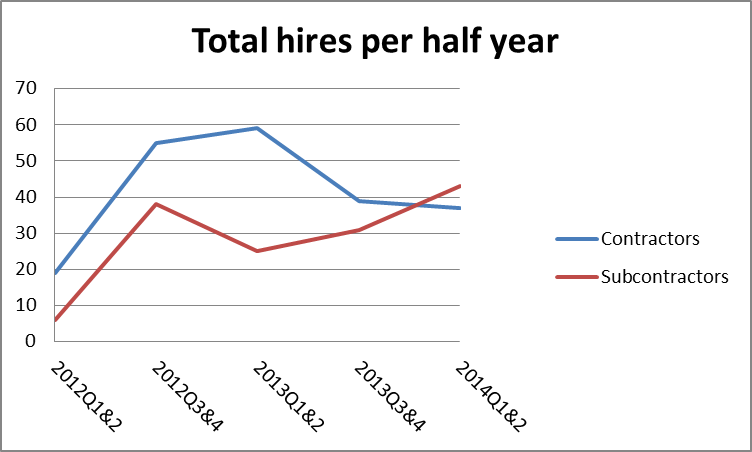
\includegraphics[width=0.45\textwidth]{appendix/total_hires_per_half_year.png}
\label{fig:total_hires_per_half_year}
%\caption{Total number of new hires per half year.}
\end{wrapfigure}
Looking at the number of new hires in Valcon we got an impression of the scope of the problem.
Even though there are some fluctuations there is a trend toward a growth in the number of hires.
This corresponds with the expressed business strategy of growth.
However, the data is not entirely conclusive, as we have only been able to look at the number of new hires within the last 30 months.
A table with all the numbers of new hires can be found in appendix \ref{app:recruitment_data} together with additional graphs.